\chapter{Pohitritev izvajanja JavaScript\\ aplikacij}
\label{sec:asm}
Prednost spletnih tehnologij je podprtost na večini platform in preprostost pisanja aplikacij z uporabo tehnologij HTML in CSS. Glavna pomanjkljivost pa je v hitrosti izvajanja JavaScript izvorne kode. Zaradi dinamičnih lastnosti jezika JavaScript obstajajo omejitve pri pohitritvi programov. Ker je hitrost izvajanja pri grafičnih aplikacijah ključnega pomena, si bomo ogledali Asm.js. Asm.js je podmnožica JavaScripta, ki lahko pospeši izvajanje programa v podprtih spletnih brskalnikih.

\section{Asm.js}

Asm.js \cite{asm} je nastal kot raziskovalni projekt pri Mozilli. Izvorno kodo JavaScripta je zaradi dinamičnosti jezika zelo težko optimizirati v modernih brskalnikih. Asm.js specifikacijo jezika omeji tako, da brskalniki kodo lažje optimizirajo. Cilj projekta je tudi dokumentirati možne pospešitve JavaScript izvorne kode.

\begin{figure}
\begin{center}
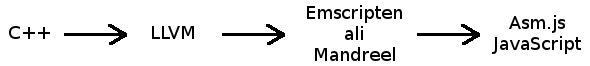
\includegraphics[width=12.5cm]{pic/emscr.png}
\end{center}
\caption{Prikaz prevajanja C++ programa v JavaScript s pomočjo prevajalnikov Emscripten in Mandreel.}
\label{emscr}
\end{figure} 

Asm.js ni novost. C++ prevajalnika Emscripten in Mandreel že znata generirati JavaScript kodo, ki jo definira Asm.js. Potek prevajanja je prikazan na sliki \ref{emscr}. Zaledje, ki ga uporabljata Emscripten in Mandreel sta ponazarjanje spomina s samostojno instanco (angl. singleton) tipiziranega spomina in uporaba bitnih operatorjev za spremenljivke, ki se obnašajo kot cela števila v C++.

Asm.js ni prvi projekt, ki iz različnih jezikov generira JavaScript izvorno kodo. Leta 2006 je podjetje Google izdalo Google Web Toolkit (GWT), ki poleg drugih stvari, prevaja izvorno kodo iz programskega jezika Java v JavaScript. Od leta 2006 se je pojavilo kar nekaj podobnih prevajalnikov za že obstoječe programske jezike (C++, C\#), kot tudi za nove jezike kot so na primer CoffeeScript, TypeScript in Dart.

Problem projektov kot je GWT je v tem, da ni standardne dokumentacije, ki bi razvijalcem JavaScript pogonov omogočilo optimizacije. Zato je tudi na primer znano, da GWT aplikacije v brskalniku Google Chrome tečejo malce hitreje kot v drugih brskalnikih. Razlog je v tem, da sta tako GWT in Chrome razvita pod isto streho in je veliko več interne komunikacije. Le-te pa ostali brskalniki niso deležni. Asm.js dokumentira vse možne pohitritve in navodila za pohitritve da na voljo vsem razvijalcem brskalnikov.

Asm.js se izogiba potencialnih upočasnitev v kodi tako, da nima spremenljivk z mešanimi tipi (angl. mixed types). Ime knjižnice izvira v dejstvu, da Asm.js izvorna koda izvaja zgolj nizko nivojske izračune, ki so podobni tistim, ki jih izvajajo zbirniki. Takšno okolje je pravšnje za zadnji del zaledja za programska jezika C in C++.

Asm.js poskrbi za precej optimizacij v času izvajanja:

\begin{itemize}
\item Tipi spremenljivk se pokažejo med preverjanjem tipov. To omogoča prevajanje pred časom in ne samo ob pravem času.
\item JavaScript pogon ima garancijo, da se tipi spremenljivk med izvajanjem ne bodo spreminjali. S tem lahko pogon proizvede bolj preprosto in bolj učinkovito kodo. 
\item Sistem tipov v Asm.js olajša globalno strukturiranje programa (klici funkcij, dostop do spomina).
\end{itemize}

Izvorna koda, ki jo definira Asm.js, je še vedno dvakrat počasnejša od domorodne kode napisane v nižje nivojskih jezikih kot sta C in C++, vendar se bo s časoma Asm.js še izboljšal.

Ker je Asm.js koda podmnožica JavaScripta lahko že danes teče v vseh brskalnikih, vendar ni nobene garancije, da bodo brskalniki pohitritve znali tudi izkoristiti.

Asm.js trenutno podpira prevajanje iz več jezikov, vendar sta popolnoma podprta samo jezika C in C++. Drugi jeziki so podprti le deloma in niso deležni enakih pohitritev in optimizacij.

Dinamični jeziki, kot so Python, Ruby in Lua, so še v zgodnjih fazah razvoja in potrebujejo še veliko dela preden bodo uporabni.

Programska jezika Java in C\# sta problematična za Asm.js, saj veliko optimizacij naredita pripadajoča navidezna stroja (JVM, .NET). Navidezna stroja optimizirata izvorno kodo na nivoju bajt kode. Te optimizacije se izgubijo, če prevajalnik prevaja iz izvorne kode v izvorno kodo. Edin način kako dobiti boljše pohitritve v teh jezikih je prevajanje celotnih navideznih strojev. To je edini način za izvajanje večine jezikov s perfektno semantiko in maksimalno hitrostjo.

Kljub omejitvam pri prevajanju dinamičnih jezikov in jezikov na virtualnih strojev, je Asm.js zelo perspektiven projekt, ki bo zaradi svoje odprtosti vsekakor pripomogel k hitrejšemu izvajanju JavaScript kode znotraj brskalnikov.
% http://kripken.github.io/mloc_emscripten_talk/\#/40
% http://mozakai.blogspot.com/2013/06/what-asmjs-is-and-what-asmjs-isnt.html
